Dado que en los sistemas biológicos las partículas se encuentran aleatoriamente orientadas, es de gran utilidad considerar las secciones transversales promedio $\langle C_{abs}\rangle$ y $\langle C_{sca}\rangle$, que son independientes de la polarización de la luz incidente, \footnote{Considerando que las partículas no sean ópticamente activas.} éstas están dadas por \cite{Bohren}:
\begin{align*}
	\langle C_{abs}\rangle &= \frac{k}{3} \text{Im}\{\alpha^{(1)}+\alpha^{(2)}+\alpha^{(3)}\},\\
	\langle C_{sca}\rangle &= \frac{k^4}{3(6\pi)} \text{Im}\{\alpha^{(1)}+\alpha^{(2)}+\alpha^{(3)}\}.
\end{align*}

En este trabajo se realizaron los cálculos para elipsoides oblatos, por lo cual, debido a la simetría del elipsoide, se satisface que $C_{ext}^{(1)}=C_{ext}^{(2)}$. 

\begin{figure}[h!]
	\sidesubfloat[]{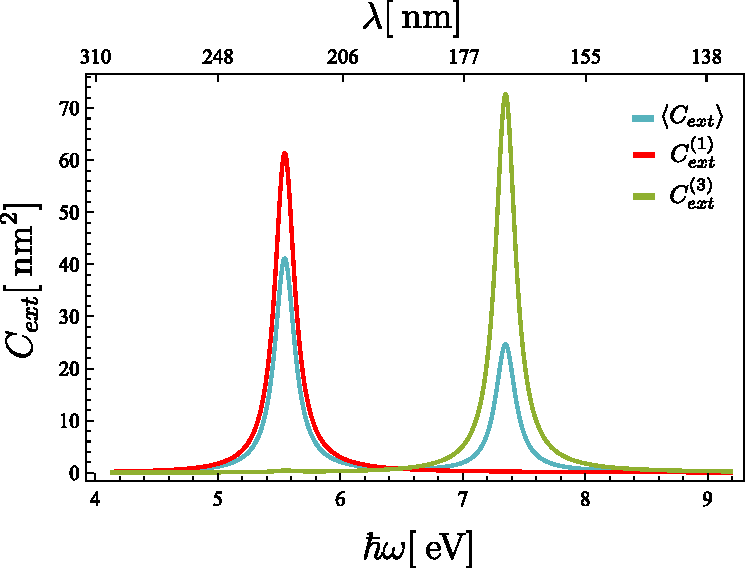
\includegraphics[width=.445\textwidth]{../../Figuras/CextAlbueno} \label{Cextpromedio}}\quad%
	\sidesubfloat[]{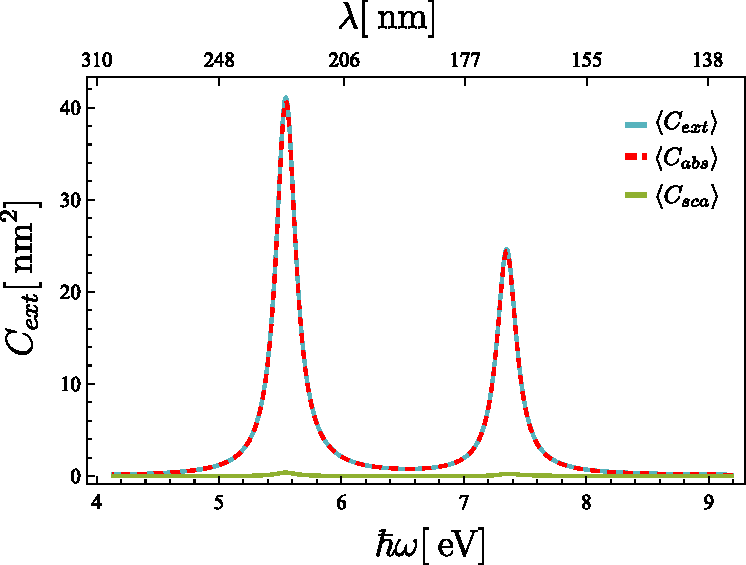
\includegraphics[width=.44\textwidth]{../../Figuras/AlContribuciones3}\label{Contribuciones}}%
	\caption{Secciones transversales como función de la energía $\hbar\omega$ y de la longitud de onda $\lambda$ para una partícula elipsoidal oblata de aluminio caracterizada por su función dieléctrica dada por el modelo de Drude ($\hbar\omega_p=13.142\text{ eV}$, $\hbar\gamma=0.197\text{ eV}$), con semiejes $a=b=1.5\text{ nm}$, $c=1\text{ nm}$ e inmersa en agua ($n_m=1.33$). \textbf{a)} Sección transversal de extinción promedio $\langle C_{ext}\rangle$, $C_{ext}^{(1)}$  y $C_{ext}^{(3)}$. \textbf{b)} Sección transversal de extinción promedio $\langle C_{ext}\rangle$ , sección transversal de absorción promedio $\langle C_{abs}\rangle$ y sección transversal de esparcimiento promedio $\langle C_{sca}\rangle$.} \label{fig:test}
\end{figure}

 En la Fig. \ref{Cextpromedio}, dado que se trata de un elipsoide oblato, al considerar $\langle C_{ext}\rangle$ se observan dos frecuencias en las que la sección transversal es máxima, las cuales coinciden con las frecuencias asociadas a $C_{ext}^{(1)}$ y $C_{ext}^{(3)}$ cuando éstas se maximizan. En la Fig. \ref{Contribuciones} se observa que en partículas pequeñas, la absorción tiene una contribución mayor en la extinción que el esparcimiento.

A continuación se presentan los cálculos de las secciones tranversales de extinción para aluminio, plata, oro, bismuto y óxido de magnesio.



\subsection*{Aluminio y plata}
En la Fig. \ref{aluminio} y \ref{plata} se observan las secciones transversales de extinción promedio para partículas de aluminio y plata, respectivamente. En las Figs. \ref{aluminioAR} y \ref{plataAR} se consideraron partículas con relación de aspecto AR$=2$ constante, en ambas figuras se observan dos máximos locales correspondientes a las frecuencias a las cuales $C_{ext}$ se maximiza al iluminar la partícula en la dirección $\hat{e}_x$ (aluminio: $254\text{ nm}$, plata: $434\text{ nm}$) y $\hat{e}_z$ (aluminio: $\lambda=146\text{ nm}$ , plata: $\lambda=344\text{ nm}$ ).  En las Figs. \ref{aluminioAR}  y \ref{plataAR} se observan las secciones transversales de extinción promedio para partículas de aluminio y plata, respectivamente, con una relación de aspecto variable; se observa que conforme la relación de aspecto se aproxima a la unidad, hay un corrimiento de las frecuencias asociadas a las $\langle C_{ext}\rangle$ máximas hacia la frecuencia de resonancia ($201\text{ nm}$) asociada a una esfera  inmersa en agua.

\begin{figure}[h!]
	\sidesubfloat[]{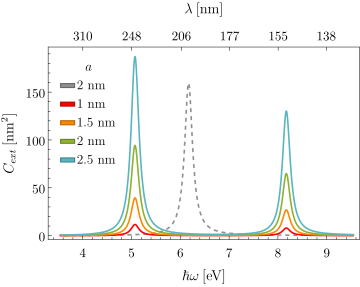
\includegraphics[width=.445\textwidth]{../../Figuras/AlAR} \label{aluminioAR}}\quad%
	\sidesubfloat[]{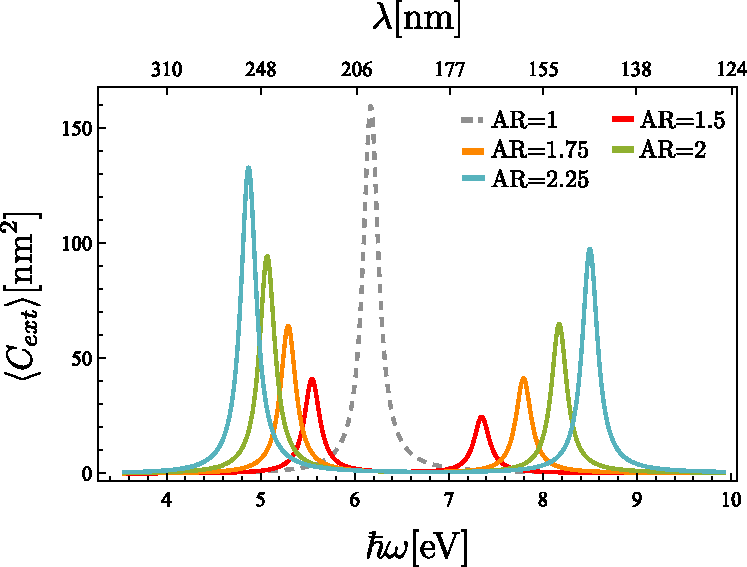
\includegraphics[width=.44\textwidth]{../../Figuras/Alc}\label{aluminioc}}%
	\caption{Secciones transversales de extinción promedio $\langle C_{ext}\rangle$ como función de la energía $\hbar\omega$ y de la longitud de onda $\lambda$ para una partícula elipsoidal oblata de aluminio caracterizada por su función dieléctrica dada por el modelo de Drude ($\hbar\omega_p=13.142\text{ eV}$, $\hbar\gamma=0.197\text{ eV}$) e inmersa en agua ($n_m=1.33$). \textbf{a)} Razón de aspecto $AR=2$ constante, excepto en el caso de una esfera (línea gris punteada) donde $AR=1$. \textbf{b)} Semieje menor $c=1$ nm constante.}\label{aluminio}}
\end{figure}

\begin{figure}[h!]
	\sidesubfloat[]{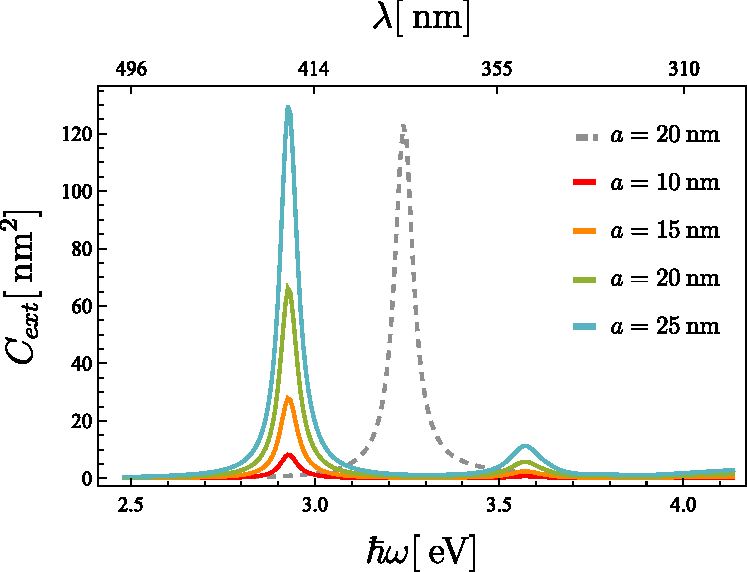
\includegraphics[width=.445\textwidth]{../../Figuras/AgAR} \label{plataAR}}\quad%
	\sidesubfloat[]{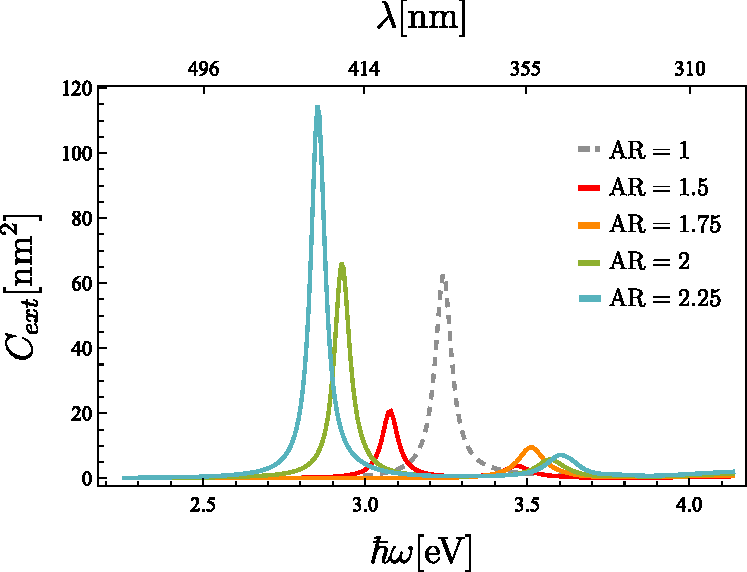
\includegraphics[width=.44\textwidth]{../../Figuras/Agc}\label{platac}}%
	\caption{Secciones transversales de extinción promedio $\langle C_{ext}\rangle$ como función de la energía $\hbar\omega$ y de la longitud de onda $\lambda$ para una partícula elipsoidal oblata de plata, cuyo índice de refracción complejo fue obtenido a partir de datos experimentales  e inmersa en agua ($n_m=1.33$). \textbf{a)} Razón de aspecto $AR=2$ constante, excepto en el caso de una esfera (línea gris punteada) donde $AR=1$. \textbf{b)} Semieje menor $c=1$ nm constante. nm}\label{plata}
\end{figure}

\subsection*{Oro y bismuto}
En la Fig. \ref{oro} se observan las secciones transversales de extinción promedio para partículas de oro, así como la parte imaginaria y real de su función dieléctrica. En la Fig. \ref{oroAR} se consideraron partículas con relación de aspecto AR$=2$ y en la Fig. \ref{oroc} se consideraron partículas con relación de aspecto variable; se observa que conforme la relación de aspecto se aproxima a la unidad, hay un corrimiento de las frecuencias asociadas a las $\langle C_{ext}\rangle$ máximas hacia la frecuencia de resonancia ($557\text{ nm}$) asociada a una esfera  inmersa en agua. Sin embargo, esta frecuencia de resonancia no se puede asociar a una frecuencia de resonancia plasmónica
no necesariamente se deben de ver dos resonancias en este caso, las resonancias no solo deben de ser de tipo Drude  , recorda el comprtamiento de lorentzianas y drude.


\begin{figure}[H]
	\sidesubfloat[]{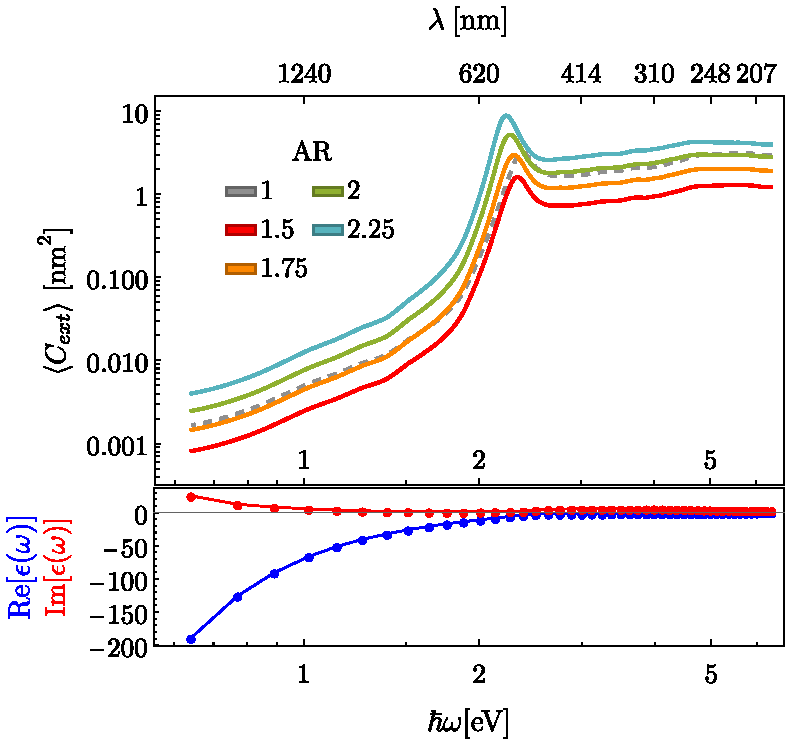
\includegraphics[width=.445\textwidth]{../../Figuras/Au} \label{oroAR}}\quad%
	\sidesubfloat[]{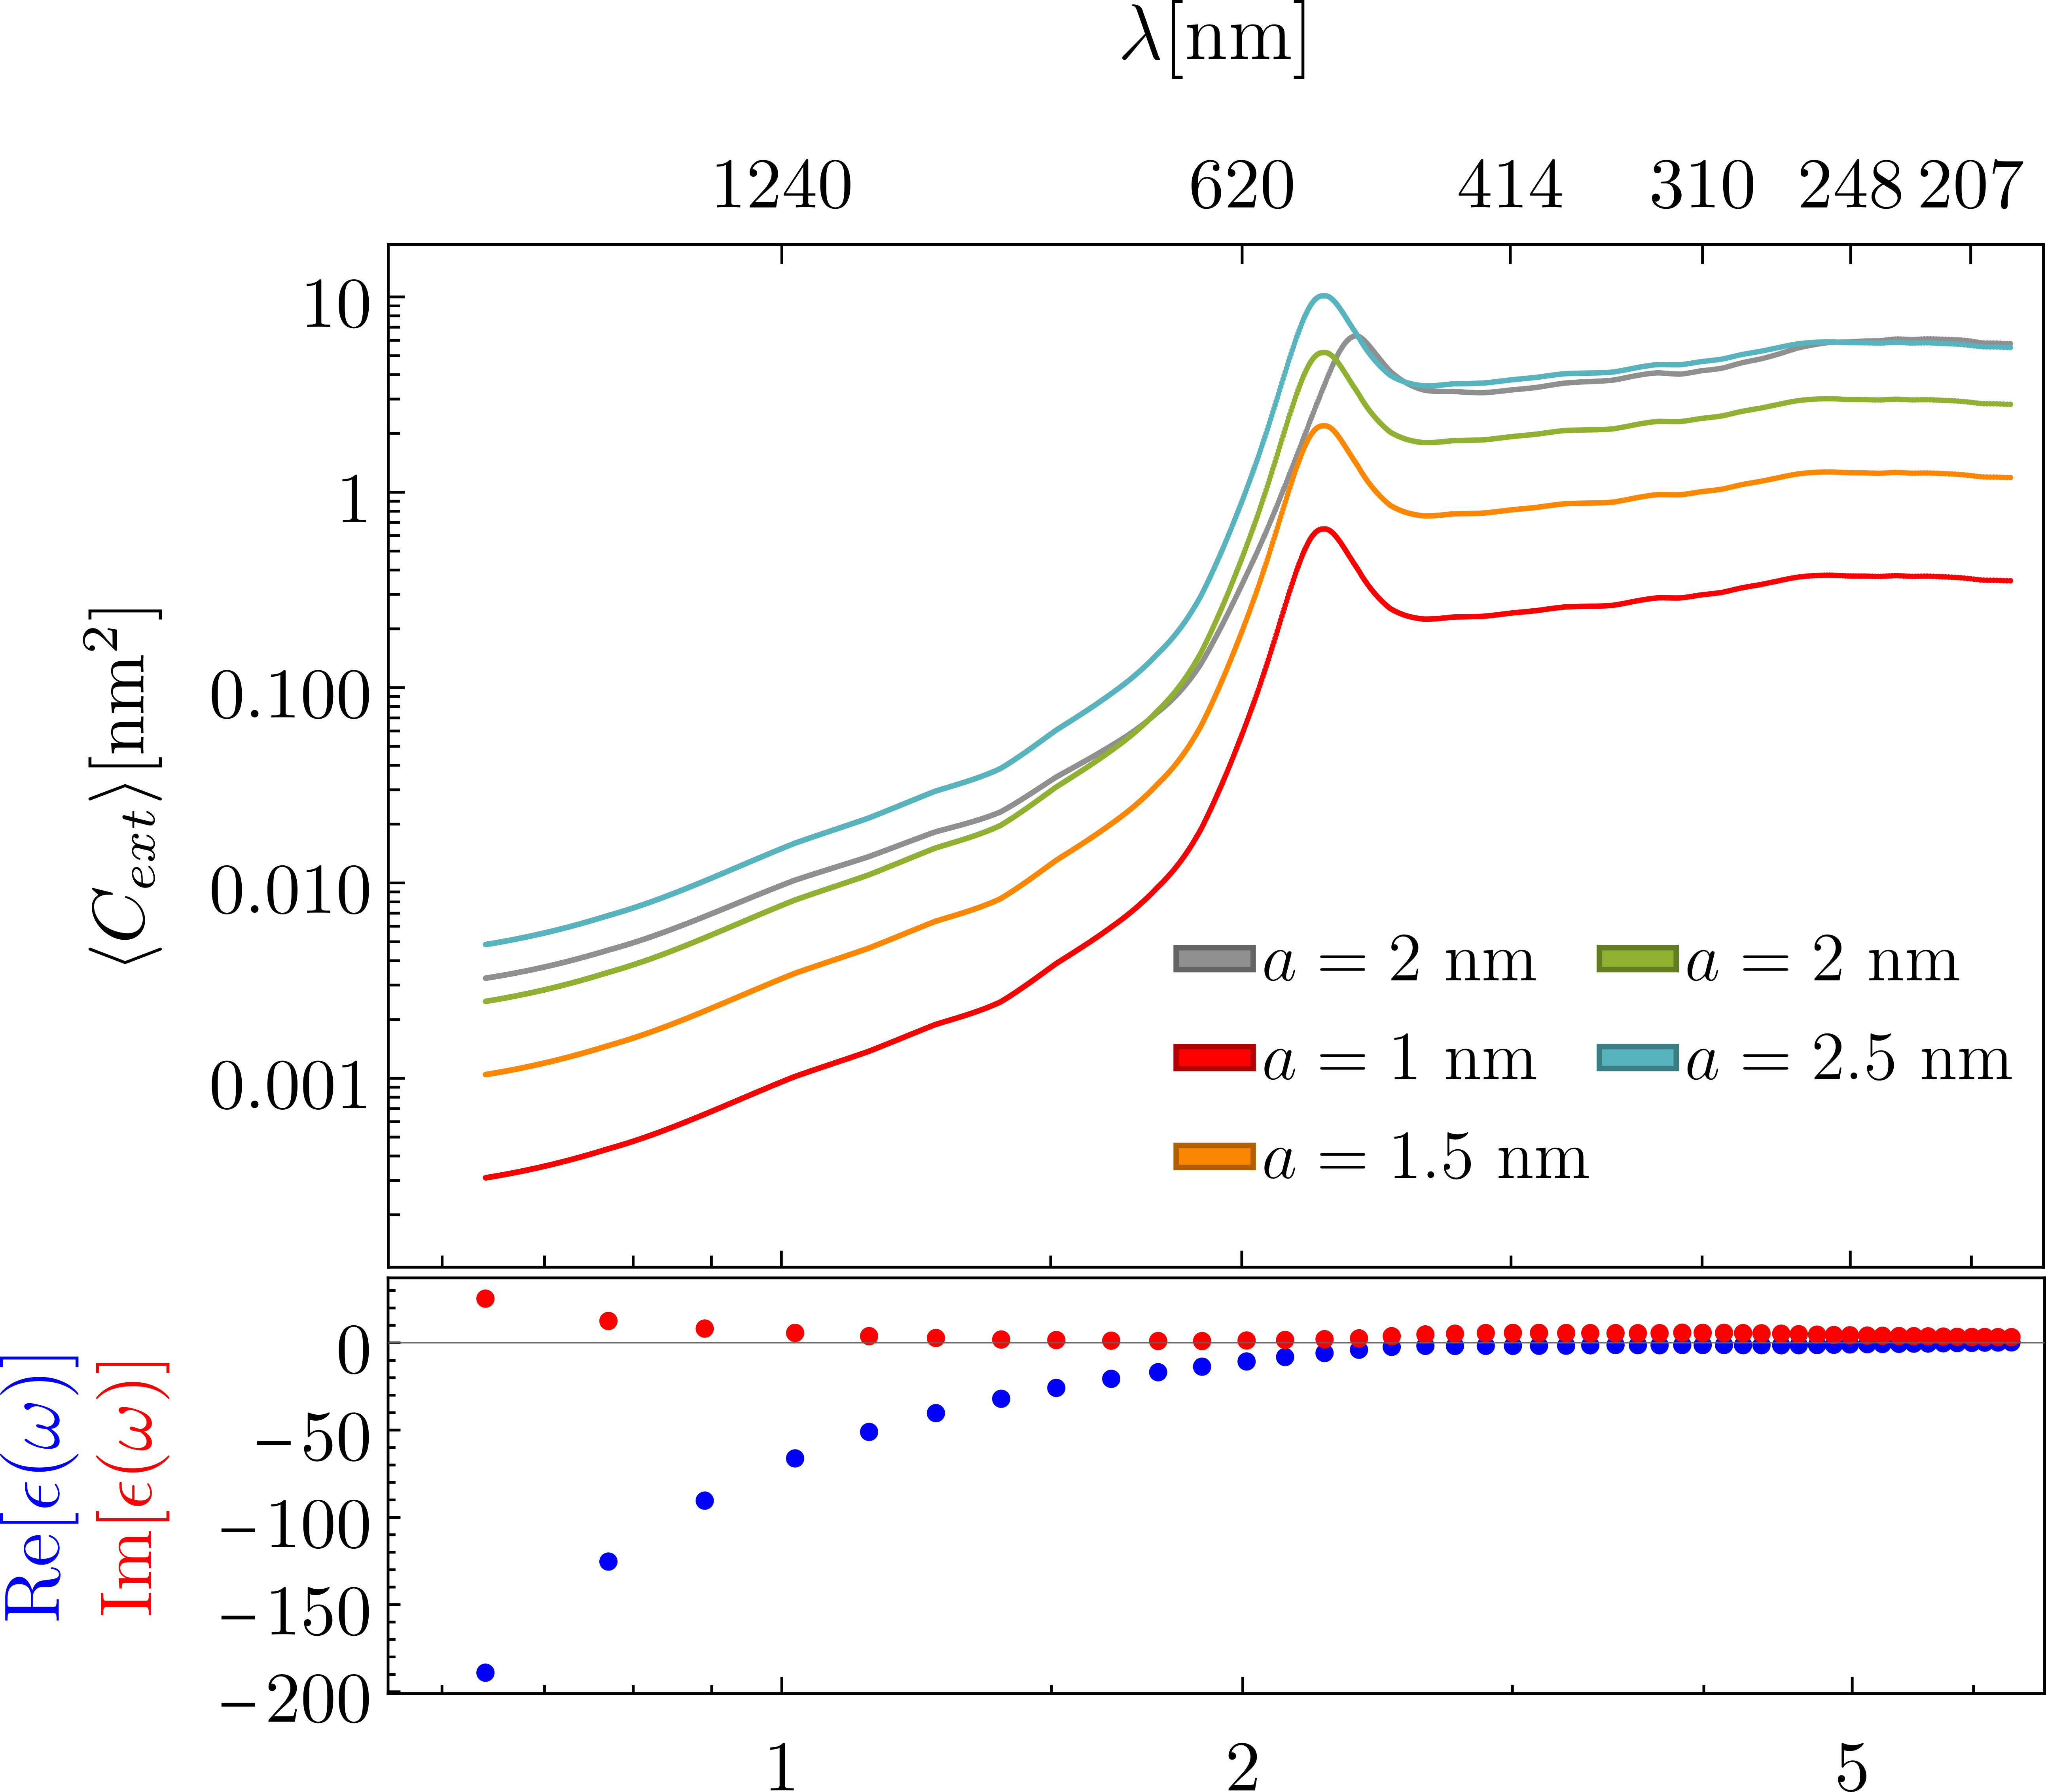
\includegraphics[width=.44\textwidth]{../../Figuras/Au2}\label{oroc}}%
	\caption{Secciones transversales de extinción promedio $\langle C_{ext}\rangle$ como función de la energía $\hbar\omega$ y de la longitud de onda $\lambda$ para una partícula elipsoidal oblata de oro, cuyo índice de refracción complejo fue obtenido a partir de datos experimentales  e inmersa en agua ($n_m=1.33$) y curvas de comparación del índice de refracción (parte real en azul, parte imaginaria en rojo) como función de la energía $\hbar\omega$ y de la longitud de onda $\lambda$ para el oro. \textbf{a)} Razón de aspecto $AR=2$ constante, excepto en el caso de una esfera (línea gris punteada) donde $AR=1$. \textbf{b)} Semieje menor $c=1$ nm constante.}\label{oro}
\end{figure}


En la Fig. \ref{bismuto} se observan las secciones transversales de extinción promedio para partículas de bismuto, así como la parte imaginaria y real de su índice de refracción. En la Fig. \ref{bismutoAR} se consideraron partículas con relación de aspecto AR$=2$  y en la Fig. \ref{bismutoc} se consideraron partículas con relación de aspecto variable.

\begin{figure}[H]
	\sidesubfloat[]{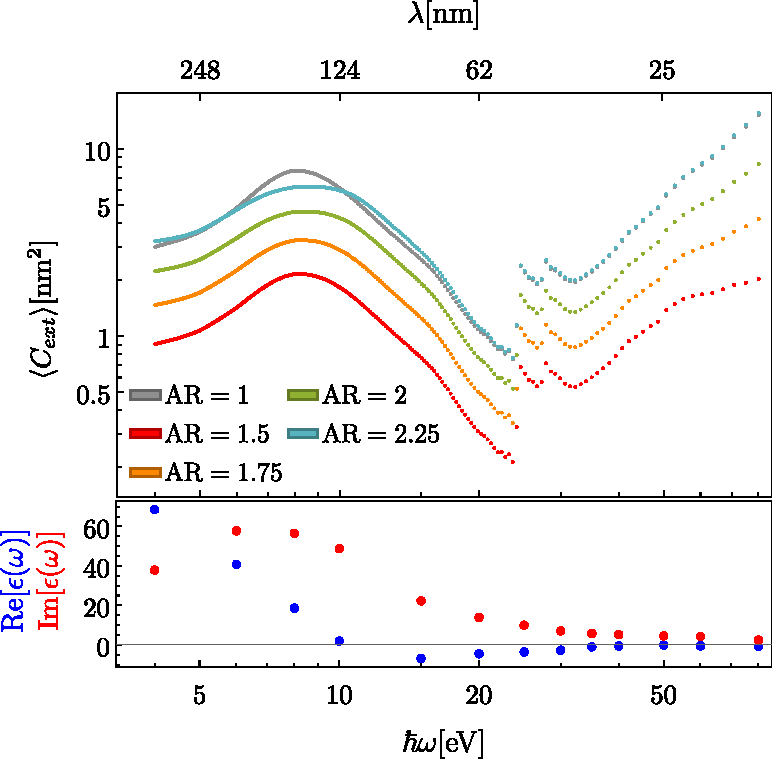
\includegraphics[width=.445\textwidth]{../../Figuras/Bi} \label{bismutoAR}}\quad%
	\sidesubfloat[]{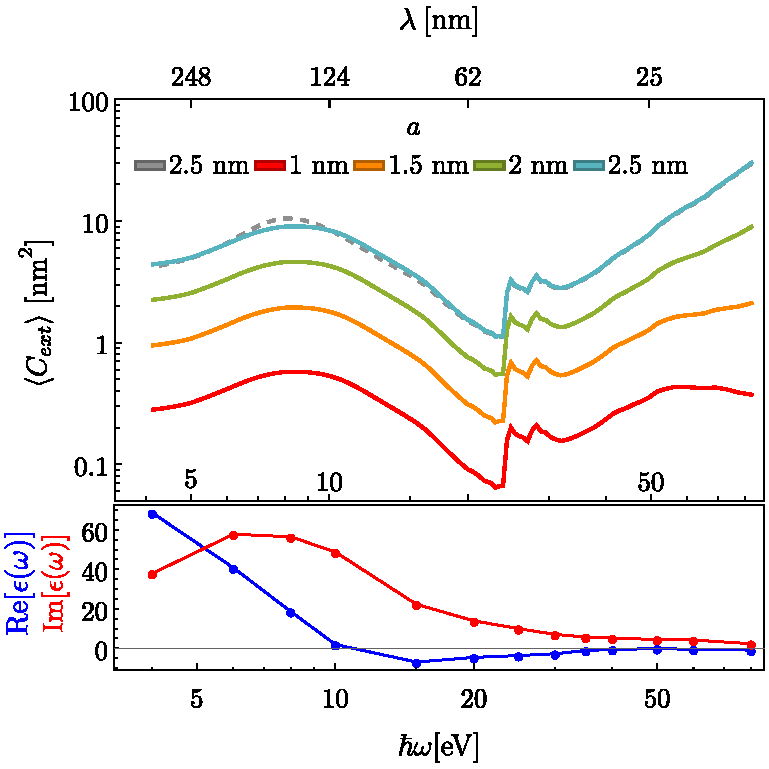
\includegraphics[width=.44\textwidth]{../../Figuras/Bi2}\label{bismutoc}}%
	\caption{Secciones transversales de extinción promedio $\langle C_{ext}\rangle$ como función de la energía $\hbar\omega$ y de la longitud de onda $\lambda$ para una partícula elipsoidal oblata de bismuto, cuyo índice de refracción complejo fue obtenido a partir de datos experimentales  e inmersa en agua ($n_m=1.33$) y curvas de comparación de la función dieléctrica (parte real en azul, parte imaginaria en rojo) como función de la energía $\hbar\omega$ y de la longitud de onda $\lambda$ para el bismuto. \textbf{a)} Razón de aspecto $AR=2$ constante, excepto en el caso de una esfera (línea gris punteada) donde $AR=1$. \textbf{b)} Semieje menor $c=1$ nm constante.}\label{bismuto}
\end{figure}


\subsection*{Óxido de magnesio}

\begin{figure}[H]
	\sidesubfloat[]{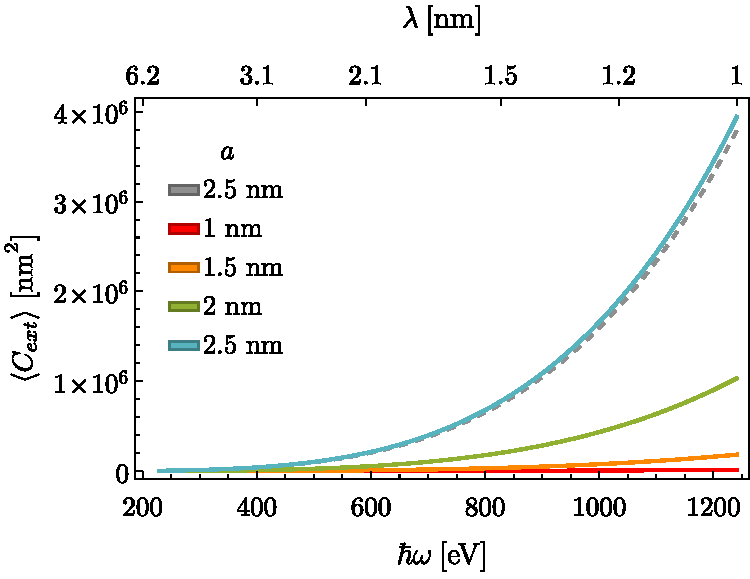
\includegraphics[width=.445\textwidth]{../../Figuras/MgOAR} \label{fig:sub1}}\quad%
	\sidesubfloat[]{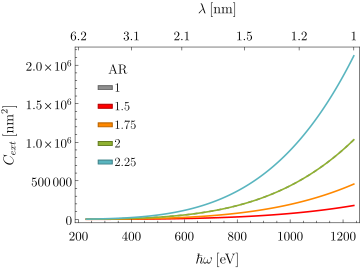
\includegraphics[width=.44\textwidth]{../../Figuras/MgOc}\label{fig:sub2}}%
	\caption{Secciones transversales de extinción promedio $\langle C_{ext}\rangle$ como función de la energía $\hbar\omega$ y de la longitud de onda $\lambda$ para una partícula elipsoidal oblata de óxido de magnesio, cuyo índice de refracción complejo fue obtenido a partir de datos experimentales  e inmersa en agua ($n_m=1.33$) y curvas de comparación de la función dieléctrica (parte real en azul, parte imaginaria en rojo) como función de la energía $\hbar\omega$ y de la longitud de onda $\lambda$ para el bismuto. \textbf{a)} Razón de aspecto $AR=2$ constante, excepto en el caso de una esfera (línea gris punteada) donde $AR=1$. \textbf{b)} Semieje menor $c=1$ nm constante.}\label{fig:test}
\end{figure}






